%~~~~~~~~~~~~~~~~~~~~~~~~~~~~~~~~~~~~~~~~~~~~~~~~~~~~~~~~~~~~~~~~~~~~~~~~~~~~~~~~~
%						GENRAL SETTINGS OF THE DOCUMENT
%~~~~~~~~~~~~~~~~~~~~~~~~~~~~~~~~~~~~~~~~~~~~~~~~~~~~~~~~~~~~~~~~~~~~~~~~~~~~~~~~~
% !TeX spellcheck = en_US
% !TeX encoding = UTF-8
% !TeX program = xelatex
\documentclass[11pt,a4paper,oneside]{report} % Single-side
%\documentclass[11pt,a4paper,twoside,openright]{report} % Duplex
% thanks to http://tex.stackexchange.com/a/47579/71109
\usepackage{ifxetex}
\usepackage{ifluatex}
\newif\ifxetexorluatex % a new conditional starts as false
\ifnum 0\ifxetex 1\fi\ifluatex 1\fi>0
   \xetexorluatextrue
\fi

\ifxetexorluatex
  \usepackage{fontspec}
\else
  \usepackage[T1]{fontenc}
  \usepackage[utf8]{inputenc}
  \usepackage[lighttt]{lmodern}
\fi

\usepackage[english,magyar]{babel} % By default, the last defined language will be active, but we will set the active language separately later.

%\usepackage{cmap}
\usepackage{amsfonts,amsmath,amssymb} % Mathematical symbols.
%\usepackage[ruled,boxed,resetcount,linesnumbered]{algorithm2e} % For pseudocodes. % beware: this is not compatible with LuaLaTeX, see http://tex.stackexchange.com/questions/34814/lualatex-and-algorithm2e
\usepackage{booktabs} % For publication quality tables for LaTeX
\usepackage{graphicx}

%\usepackage{fancyhdr}
%\usepackage{lastpage}

\usepackage{anysize}
%\usepackage{sectsty}
\usepackage{setspace} % For setting line spacing

\usepackage[unicode]{hyperref} % For hyperlinks in the generated document.
\usepackage{xcolor}
\usepackage{listings} % For source code snippets.

\usepackage[amsmath,thmmarks]{ntheorem} % Theorem-like environments.

\usepackage[hang]{caption}

\singlespacing

\newcommand{\selecthungarian}{
	\selectlanguage{magyar}
	\setlength{\parindent}{2em}
	\setlength{\parskip}{0em}
	\frenchspacing
}

\newcommand{\selectenglish}{
	\selectlanguage{english}
	\setlength{\parindent}{0em} % orginal was 0 and 0.5
	\setlength{\parskip}{0.5em}
	\nonfrenchspacing
	\renewcommand{\figureautorefname}{Figure}
	\renewcommand{\tableautorefname}{Table}
	\renewcommand{\partautorefname}{Part}
	\renewcommand{\chapterautorefname}{Chapter}
	\renewcommand{\sectionautorefname}{Section}
	\renewcommand{\subsectionautorefname}{Section}
	\renewcommand{\subsubsectionautorefname}{Section}
}

\usepackage[numbers]{natbib}
\usepackage{xspace}
\newcommand{\vikszerzoVezeteknev}{Erbasi} %Author
\newcommand{\vikszerzoKeresztnev}{Türker}
\newcommand{\vikkonzulensAMegszolitas}{Dr.~} %Advisor #1
\newcommand{\vikkonzulensAVezeteknev}{Vizer}
\newcommand{\vikkonzulensAKeresztnev}{Dániel}
\newcommand{\vikkonzulensBMegszolitas}{Dr.~} %Advisor #2
\newcommand{\vikkonzulensBVezeteknev}{Kiss}
\newcommand{\vikkonzulensBKeresztnev}{Bálint}
\newcommand{\vikkonzulensCMegszolitas}{} %Advisor #3
\newcommand{\vikkonzulensCVezeteknev}{}
\newcommand{\vikkonzulensCKeresztnev}{}
\newcommand{\vikcim}{Affine Parameter-Dependent Lyapunov Stability Analysis of Electronic Power Steering Systems} %Title
\newcommand{\viktanszek}{\bmeiit}%Department
\newcommand{\vikdoktipus}{\bsc} %Document type (\bsc or \msc)
\newcommand{\vikmunkatipusat}{} %For the "student declaration" section: thesis
\newcommand{\szerzoMeta}{\vikszerzoVezeteknev{} \vikszerzoKeresztnev} % One author
%--------------------------------------------------------------------------------------
% Elnevezések
%--------------------------------------------------------------------------------------
\newcommand{\bme}{Budapest University of Technology and Economics}
\newcommand{\vik}{Faculty of Electrical Engineering and Informatics}

\newcommand{\bmeiit}{Department of Control Engineering and Information Technology}

\newcommand{\keszitette}{Author}
\newcommand{\konzulens}{Advisor}

\newcommand{\bsc}{Bachelor's Thesis}
\newcommand{\msc}{Master's Thesis}
\newcommand{\tdk}{Scientific Students' Association Report}
\newcommand{\bsconlab}{BSc Project Laboratory}
\newcommand{\msconlabi}{MSc Project Laboratory 1}
\newcommand{\msconlabii}{MSc Project Laboratory 2}

\newcommand{\pelda}{Example}
\newcommand{\definicio}{Definition}
\newcommand{\tetel}{Theorem}

\newcommand{\bevezetes}{Introduction}
\newcommand{\koszonetnyilvanitas}{Acknowledgments}
\newcommand{\fuggelek}{Appendix}

% Optional custom titles
%\addto\captionsenglish{%
%\renewcommand*{\listfigurename}{Your list of figures title}
%\renewcommand*{\listtablename}{Your list of tables title}
%\renewcommand*{\bibname}{Your bibliography title}
%}

\newcommand{\szerzo}{\vikszerzoKeresztnev{} \vikszerzoVezeteknev}
\newcommand{\vikkonzulensA}{\vikkonzulensAMegszolitas\vikkonzulensAKeresztnev{} \vikkonzulensAVezeteknev}
\newcommand{\vikkonzulensB}{\vikkonzulensBMegszolitas\vikkonzulensBKeresztnev{} \vikkonzulensBVezeteknev}
\newcommand{\vikkonzulensC}{\vikkonzulensCMegszolitas\vikkonzulensCKeresztnev{} \vikkonzulensCVezeteknev}

\newcommand{\selectthesislanguage}{\selectenglish}

\bibliographystyle{plainnat}

\newcommand{\ie}{i.e.\@\xspace}
\newcommand{\Ie}{I.e.\@\xspace}
\newcommand{\eg}{e.g.\@\xspace}
\newcommand{\Eg}{E.g.\@\xspace}
\newcommand{\etal}{et al.\@\xspace}
\newcommand{\etc}{etc.\@\xspace}
\newcommand{\vs}{vs.\@\xspace}
\newcommand{\viz}{viz.\@\xspace} % videlicet
\newcommand{\cf}{cf.\@\xspace} % confer
\newcommand{\Cf}{Cf.\@\xspace}
\newcommand{\wrt}{w.r.t.\@\xspace} % with respect to
\newcommand{\approximately}{approx.\@\xspace}

\newcommand{\appendixnumber}{1}  % a fofejezet-szamlalo az angol ABC 1. betuje (A) lesz
 %Settings for English documents
%--------------------------------------------------------------------------------------
% Page layout setup
%--------------------------------------------------------------------------------------
% we need to redefine the pagestyle plain
% another possibility is to use the body of this command without \fancypagestyle
% and use \pagestyle{fancy} but in that case the special pages
% (like the ToC, the References, and the Chapter pages)remain in plane style

\pagestyle{plain}
\marginsize{35mm}{25mm}{15mm}{15mm}

\setcounter{tocdepth}{3}
%\sectionfont{\large\upshape\bfseries}
\setcounter{secnumdepth}{3}

\sloppy % Margón túllógó sorok tiltása.
\widowpenalty=10000 \clubpenalty=10000 %A fattyú- és árvasorok elkerülése
\def\hyph{-\penalty0\hskip0pt\relax} % Kötőjeles szavak elválasztásának engedélyezése


%--------------------------------------------------------------------------------------
% Setup hyperref package
%--------------------------------------------------------------------------------------
\hypersetup{
    % bookmarks=true,            % show bookmarks bar?
    unicode=true,              % non-Latin characters in Acrobat's bookmarks
    pdftitle={\vikcim},        % title
    pdfauthor={\szerzoMeta},    % author
    pdfsubject={\vikdoktipus}, % subject of the document
    pdfcreator={\szerzoMeta},   % creator of the document
    pdfproducer={},    % producer of the document
    pdfkeywords={},    % list of keywords (separate then by comma)
    pdfnewwindow=true,         % links in new window
    colorlinks=true,           % false: boxed links; true: colored links
    linkcolor=black,           % color of internal links
    citecolor=black,           % color of links to bibliography
    filecolor=black,           % color of file links
    urlcolor=black             % color of external links
}


%--------------------------------------------------------------------------------------
% Set up listings
%--------------------------------------------------------------------------------------
\definecolor{lightgray}{rgb}{0.95,0.95,0.95}
\lstset{
	basicstyle=\scriptsize\ttfamily, % print whole listing small
	keywordstyle=\color{black}\bfseries, % bold black keywords
	identifierstyle=, % nothing happens
	% default behavior: comments in italic, to change use
	% commentstyle=\color{green}, % for e.g. green comments
	stringstyle=\scriptsize,
	showstringspaces=false, % no special string spaces
	aboveskip=3pt,
	belowskip=3pt,
	backgroundcolor=\color{lightgray},
	columns=flexible,
	keepspaces=true,
	escapeinside={(*@}{@*)},
	captionpos=b,
	breaklines=true,
	frame=single,
	float=!ht,
	tabsize=2,
	literate=*
		{á}{{\'a}}1	{é}{{\'e}}1	{í}{{\'i}}1	{ó}{{\'o}}1	{ö}{{\"o}}1	{ő}{{\H{o}}}1	{ú}{{\'u}}1	{ü}{{\"u}}1	{ű}{{\H{u}}}1
		{Á}{{\'A}}1	{É}{{\'E}}1	{Í}{{\'I}}1	{Ó}{{\'O}}1	{Ö}{{\"O}}1	{Ő}{{\H{O}}}1	{Ú}{{\'U}}1	{Ü}{{\"U}}1	{Ű}{{\H{U}}}1
}


%--------------------------------------------------------------------------------------
% Set up theorem-like environments
%--------------------------------------------------------------------------------------
% Using ntheorem package -- see http://www.math.washington.edu/tex-archive/macros/latex/contrib/ntheorem/ntheorem.pdf

\theoremstyle{plain}
\theoremseparator{.}
\newtheorem{example}{\pelda}

\theoremseparator{.}
%\theoremprework{\bigskip\hrule\medskip}
%\theorempostwork{\hrule\bigskip}
\theorembodyfont{\upshape}
\theoremsymbol{{\large \ensuremath{\centerdot}}}
\newtheorem{definition}{\definicio}

\theoremseparator{.}
%\theoremprework{\bigskip\hrule\medskip}
%\theorempostwork{\hrule\bigskip}
\newtheorem{theorem}{\tetel}


%--------------------------------------------------------------------------------------
% Some new commands and declarations
%--------------------------------------------------------------------------------------
\newcommand{\code}[1]{{\upshape\ttfamily\scriptsize\indent #1}}
\newcommand{\doi}[1]{DOI: \href{http://dx.doi.org/\detokenize{#1}}{\raggedright{\texttt{\detokenize{#1}}}}} % A hivatkozások közt így könnyebb DOI-t megadni.

\DeclareMathOperator*{\argmax}{arg\,max}
%\DeclareMathOperator*[1]{\floor}{arg\,max}
\DeclareMathOperator{\sign}{sgn}
\DeclareMathOperator{\rot}{rot}


%--------------------------------------------------------------------------------------
% Setup captions
%--------------------------------------------------------------------------------------
\captionsetup[figure]{
	width=.75\textwidth,
	aboveskip=10pt}

\renewcommand{\captionlabelfont}{\bf}
%\renewcommand{\captionfont}{\footnotesize\it}

%--------------------------------------------------------------------------------------
% Hyphenation exceptions
%--------------------------------------------------------------------------------------
\hyphenation{Shakes-peare Mar-seilles ár-víz-tű-rő tü-kör-fú-ró-gép}


\author{\vikszerzo}
\title{\viktitle}

%~~~~~~~~~~~~~~~~~~~~~~~~~~~~~~~~~~~~~~~~~~~~~~~~~~~~~~~~~~~~~~~~~~~~~~~~~~~~~~~~~
%						The main part of the thesis
%~~~~~~~~~~~~~~~~~~~~~~~~~~~~~~~~~~~~~~~~~~~~~~~~~~~~~~~~~~~~~~~~~~~~~~~~~~~~~~~~~
\begin{document}

\pagenumbering{gobble} %Roman numerals page numbering

\selectthesislanguage %English

%--------------------------------------------------------------------------------------
% Task DESCRIPTION (printed version available in the classrooms)
%--------------------------------------------------------------------------------------
\clearpage

\begin{flushright}

\includegraphics[width=45mm,keepaspectratio]{figures/tk_logo.png} \\[1cm] \end{flushright}

\begin{center}
\large
\textbf{TASK DESCRIPTION}\\[0.4cm]

\textbf{Affine Parameter-Dependent Lyapunov Stability Analysis of Electronic Power Steering Systems} \\
\end{center}

The application of electronic power steering (EPS) is mandatory for modern vehicles. Due to the increasing application of driver assistance and autonomous functions (ADAS), the steering system is a safety-critical human-machine interface. It is thus crucial to maintain the system in a stable region during operation. In order to achieve this goal, qualitative measures are needed a priori to support controller synthesis. By their nature, EPS systems have a couple of nonlinearities. However, they can be approximated by linear parameter-varying (LPV) models where the scheduling variables capture the nonlinear effects. Based on the LPV model, a stabilizing full-state feedback controller can be designed. The design can be effectively supported by the aforementioned qualitative measures of regions of stability in the parameter space.

This project work aims at quantifying the parameter-varying stability region of EPS for further ADAS interface development. The tasks of the student will be:
\begin{enumerate}
	\item Literature study of affine LPV models and their quadratic stability in general;
	\item Development of an affine LPV model for the EPAS system based on the literature;
	\item Development of a set of affine parameter-dependent Lyapunov functions for the EPAS system;
	\item Analysis of the quadratic stability regions of the EPAS system; 
\end{enumerate}

For the completion of this project work the Thyssenkrupp Component Technology Hungary Kft. assures the supervisor and the necessary equipment.

Supervisor: Dr. Dániel Vizer,  daniel.vizer@thyssenkrupp.com. %Task description

\hypersetup{pageanchor=false}
%~~~~~~~~~~~~~~~~~~~~~~~~~~~~~~~~~~~~~~~~~~~~~~~~~~~~~~~~~~~~~~~~~~~~~~~~~~~~~~~~~
%								The title page

\begin{titlepage}
\begin{center}

\includegraphics[width=60mm,keepaspectratio]{figures/bme_logo.pdf}
\hspace{5mm}

\includegraphics[width=60mm,keepaspectratio]{figures/tk_logo.png}
\\[0.3cm]
$\vcenter{\hbox{
\includegraphics[width=24mm,keepaspectratio]{figures/vik_logo.png}}}$
\hspace{10mm}
$\vcenter{\hbox{
\includegraphics[width=16mm,keepaspectratio]{figures/iit_logo.png}}}$
\\[0.4cm]

\textbf{\bme}\\
\textmd{\vik}\\
\textmd{\viktanszek}\\[4cm]

\vspace{0.4cm}
{\huge \bfseries \vikcim}\\[0.8cm]
\vspace{0.5cm}
\textsc{\Large \vikdoktipus}\\[4cm]

{
	\renewcommand{\arraystretch}{0.85}
	\begin{tabular}{cc}
	 \makebox[7cm]{\emph{\keszitette}} & \makebox[7cm]{\emph{\konzulens}} \\ \noalign{\smallskip}
	 \makebox[7cm]{\szerzo} & \makebox[7cm]{\vikkonzulensA} \\
	  & \makebox[7cm]{\vikkonzulensB} \\
	  & \makebox[7cm]{\vikkonzulensC} \\
	\end{tabular}
}

\vfill
{\large \today}
\end{center}
\end{titlepage}
\hypersetup{pageanchor=false} %Thesis title page

\tableofcontents\vfill %Table of Contents

\selectlanguage{english}
\pagenumbering{gobble}
%~~~~~~~~~~~~~~~~~~~~~~~~~~~~~~~~~~~~~~~~~~~~~~~~~~~~~~~~~~~~~~~~~~~~~~~~~~~~~~~~~
% 								DECLARATION

\begin{center}
\large
\textbf{STUDENT DECLARATION}\\
\end{center}

I, \emph{\vikszerzoVezeteknev{} \vikszerzoKeresztnev}, the undersigned, hereby declare that the present \vikdoktipus{} work has been prepared by myself and without any unauthorized help or assistance. Only the specified sources (references, tools, etc.) were used. All parts taken from other sources word by word, or after rephrasing but with identical meaning, were unambiguously identified with explicit reference to the sources utilized.

I authorize the Faculty of Electrical Engineering and Informatics of the Budapest University of Technology and Economics to publish the principal data of the thesis work (author's name, title, abstracts in English and in a second language, year of preparation, supervisor's name, etc.) in a searchable, public, electronic and online database and to publish the full text of the thesis work on the internal network of the university (this may include access by authenticated outside users). I declare that the submitted hard-copy of the thesis work and its electronic version are identical. 

\begin{flushleft}
\vspace*{1cm}
Budapest, \today
\end{flushleft}

\begin{flushright}
 \vspace*{1cm}
 \makebox[7cm]{\rule{6cm}{.4pt}}\\
 \makebox[7cm]{\emph{\vikszerzoVezeteknev{} \vikszerzoKeresztnev}}\\
 \makebox[7cm]{student}
\end{flushright}
\thispagestyle{empty}

\vfill
\clearpage
\thispagestyle{empty} % an empty page

\selectthesislanguage
 %Student declaration

\pagenumbering{roman}
\setcounter{page}{1}

%~~~~~~~~~~~~~~~~~~~~~~~~~~~~~~~~~~~~~~~~~~~~~~~~~~~~~~~~~~~~~~~~~~~~~~~~~~~~~~~~~
\chapter*{\koszonetnyilvanitas}\addcontentsline{toc}{chapter}{\koszonetnyilvanitas}

Ez nem kötelező, akár törölhető is. Ha a szerző szükségét érzi, itt lehet köszönetet nyilvánítani azoknak, akik hozzájárultak munkájukkal ahhoz, hogy a hallgató a szakdolgozatban vagy diplomamunkában leírt feladatokat sikeresen elvégezze. A konzulensnek való köszönetnyilvánítás sem kötelező, a konzulensnek hivatalosan is dolga, hogy a hallgatót konzultálja.

\newcounter{romanPage}
\setcounter{romanPage}{\value{page}}
\stepcounter{romanPage} %TODO

\selectenglish

%~~~~~~~~~~~~~~~~~~~~~~~~~~~~~~~~~~~~~~~~~~~~~~~~~~~~~~~~~~~~~~~~~~~~~~~~~~~~~~~~~
%							Abstract in English
\chapter*{Abstract}\addcontentsline{toc}{chapter}{Abstract}

This document is a \LaTeX-based skeleton for BSc/MSc~theses of students at the Electrical Engineering and Informatics Faculty, Budapest University of Technology and Economics. The usage of this skeleton is optional. It has been tested with the \emph{TeXLive} \TeX~implementation, and it requires the PDF-\LaTeX~compiler.

\vfill
\selecthungarian


%~~~~~~~~~~~~~~~~~~~~~~~~~~~~~~~~~~~~~~~~~~~~~~~~~~~~~~~~~~~~~~~~~~~~~~~~~~~~~~~~~
%							Abstract in Turkish
\chapter*{{\"O}zet}\addcontentsline{toc}{chapter}{{\"O}zet}

Bu belge, Budapeşte Teknoloji ve Ekonomi Üniversitesi, Elektrik Mühendisliği ve Bilişim Fakültesi'ndeki öğrencilerin BSc/MSc~tezleri için \LaTeX-based bir iskelettir. Bu iskeletin kullanımı isteğe bağlıdır. \emph{TeXLive} \TeX~implementation'la test edilmiştir ve PDF-\LaTeX~compiler gerektirir.


\selectenglish


\vfill
\selectthesislanguage
 %TODO

%~~~~~~~~~~~~~~~~~~~~~~~~~~~~~~~~~~~~~~~~~~~~~~~~~~~~~~~~~~~~~~~~~~~~~~~~~~~~~~~~~
%							LIST OF NOTATIONS
\chapter*{Notations lists}\addcontentsline{toc}{chapter}{Lists of symbols and abbreviations}

\section*{List of symbols}
\addcontentsline{toc}{section}{List of symbols}

\begin{table}[ht]
	\centering
	\begin{tabular}[t]{c l} %c for center aligned, l for left aligned columns. 
		\toprule
			Symbol				&	Description							\\
		\midrule
			$t$ 				& 	Time variable 						\\
			$x(t)$ 				& 	States Vector						\\
			$\omega(t)$ 		& 	General disturbance	signal vector	\\
			$z(t)$ 				& 	General output signal vector		\\
			$u(t)$ 				& 	Controllable input vector	 		\\			
			$y(t)$				& 	Output vector						\\
			$p(t)$ 				& 	Time varying parameter				\\
			%
			$A$					& 	Constant system matrix 					\\
			$B$	 				& 	Constant disturbance matrix 			\\
			$C$	 				& 	Constant output matrix 					\\
			$D$					&	Constant feed-forward matrix			\\
			$\mathcal{A}(p(t))$	& 	Parameter-varying system matrix 		\\
			$\mathcal{B}(p(t))$	& 	Parameter-varying disturbance matrix	\\
			$\mathcal{C}(p(t))$	& 	Parameter-varying output matrix 		\\
			$\mathcal{D}(p(t))$	& 	Parameter-varying feed-forward matrix 	\\
			%
			$\mathbb{R}$		&	Set of real numbers					\\
			$\mathbb{Z}$		&	Set of integer numbers				\\
			$\in$				&	Is a member of						\\
			$\subseteq$			&	Is subset of						\\
			%
			$M^T$				&	Transpose of the matrix M			\\
			$M^*$				&	Complex conjugate of the matrix M	\\
			$M^{n \times m}$	&	Matrix with n rows and m columns	\\
			$\|x\|$				&	Standard Euclidean norm				\\
		\bottomrule
	\end{tabular}
	\caption{Notations used in this thesis work.}
\end{table}

%~~~~~~~~~~~~~~~~~~~~~~~~~~~~~~~~~~~~~~~~~~~~~~~~~~~~~~~~~~~~~~~~~~~~~~~~~~~~~~~~~
%						LIST OF ABBREVIATIONS
\clearpage
\section*{List of abbreviations}
\addcontentsline{toc}{section}{List of abbreviations}

\begin{table}[ht]
	\centering
	\begin{tabular}{l l}
		\toprule
			Abbreviation 	&	Description							\\
		\midrule
			LTI 			& 	Linear Time-Invariant 				\\
			LTV				& 	Linear Time-Varying 				\\
			LPV 			& 	Linear Parameter-Varying 			\\
			EPAS or EPS		&	Electric Power Assisted Steering	\\
			CT 				& 	Continuous Time 					\\
			DT				&	Discrete Time						\\
			SI 				& 	Single Input 						\\
			SO				&	Single Output						\\
			MI 				& 	Multiple Input 						\\
			MO				&	Multiple Output						\\
		\bottomrule
	\end{tabular}
	\caption{Abbreviations used in this thesis work.}
\end{table}
 %Symbol list

\pagenumbering{arabic} %Arabic numeral page numbering

%~~~~~~~~~~~~~~~~~~~~~~~~~~~~~~~~~~~~~~~~~~~~~~~~~~~~~~~~~~~~~~~~~~~~~~~~~~~~~~~~~
\chapter{\bevezetes}

The introduction contains the analysis of the diploma plan announcement, its historical antecedents, the justification of the task (description of the motivation), the solutions so far and, in light of this, a summary of the student's solution.

As usual, the introduction ends with the structure of the diploma plan, i.e. with a brief description of what each chapter deals with. %TODO

%~~~~~~~~~~~~~~~~~~~~~~~~~~~~~~~~~~~~~~~~~~~~~~~~~~~~~~~~~~~~~~~~~~~~~~~~~~~~~~~~~
\chapter{Linear parameter varying modeling and stability} 
\label{chap_linear_parameter_varying_modeling_and_stability}
% Approx. 10 pages

%~~~~~~~~~~~~~~~~~~~~~~~~~~~~~~~~~~~~~~~~~~~~~~~~~~~~~~~~~~~~~~~~~~~~~~~~~~~~~~~~~
\section{Introduction}
%TODO INTRODUCTION TO LPV SYSTEM ONLY VERBAL.


%~~~~~~~~~~~~~~~~~~~~~~~~~~~~~~~~~~~~~~~~~~~~~~~~~~~~~~~~~~~~~~~~~~~~~~~~~~~~~~~~~
\section{System classification}
\label{sec_system_classification}

Control systems can be grouped into main categories from different points of view and based on some parameters.

Based on the number of inputs and outputs. Control systems can be classified as SISO control systems or MIMO control systems. When a system has only one input, it is called a single input system and is notated with the initials SI. If it has more than one input, the system is called a multiple input system, or MI system. If a system has only one output, it is called a single output system, or SO system. If it has more than one output, it is called a multiple output system, or MO system. This way, we can refer to any system with this convention. For example, for a single input, single output system, it can be said the system is a SISO system; if it has more inputs and more outputs, it can be said it is a MIMO system, etc.

Based on the type of the signal used. Control systems can be classified as continuous-time control systems or discrete-time control systems. In continuous-time control systems, all the signals are continuous in time. However, in discrete-time control systems, there may be one or more discrete time signals.

Based on the feedback signal. Control systems can be classified as feed-forward control systems, also called open-loop control systems, or feed-back control systems, also called closed-loop control systems. Feed-forward control systems do not utilize the output signal and do not feed it back to the system for correction. \Ie, the input does not self-correct using feedback from the output. On the other hand, feed-back control systems utilize the output signal for self-correction. So, the control action depends on the output. The error detector generates an error signal that is equal to the difference between the input and feedback signals, and then this error signal is fed to the controller.

%TODO Add here a figure of a closed loop control system. general_control_sys.png

%~~~~~~~~~~~~~~~~~~~~~~~~~~~~~~~~~~~~~~~~~~~~~~~~~~~~~~~~~~~~~~~~~~~~~~~~~~~~~~~~~
\section{System representation} 
\label{sec_system_representaion}

A system may generally be thought of as an operator or transformation from the input to the output; hence, an equation can be used to describe how a system works~\citep{fazekas2010fundamentals}.

\begin{align}
	y(t) = G(u(t)) 
\end{align}

where, $u(t)$ is the input, $y(t)$ is the output and $G(\bullet)$ is the operator of the system. 

The realizable systems are \textit{causal systems}, meaning that their current outputs are independent of their potential future inputs. The output is a signal generated and measured by the system. Noise or measurement error is generally included in the measurement~\citep[Chapter~2.1.1]{fazekas2010fundamentals}.

The system is called linear if:

\begin{subequations}	
	\begin{align}
		y_1(t) = G(u_1(t)) \text{ and } y_2(t) = G(u_2(t)) 
		\\
		a_1y_1(t) + a_2y_2(t) = G(a_1u_1(t) + a_2u_2(t))
	\end{align}	
\end{subequations}

where, $a_1, a_2 \in \mathbb{R}$.

The system is called linear time-invariant if the output of the system is independent form the time of the input, \ie, if:

\begin{subequations} \label{eq_time_invariance}
	\begin{align}
		y(t) &= G(u(t)) 
		\\
		y(t - \tau) &= G(u(t - \tau)) 
	\end{align}
\end{subequations}

where, $\tau$ is the time delay, and $\tau \in \mathbb{R}$.

Equations above (\ref{eq_time_invariance}) indicates that the timing of the input has no bearing on how the system will behave; the timing of the experiment is meaningless. If the input is unchanged and the input is only time-shifted, the output is unchanged \citep{fazekas2010fundamentals}.

If the system's output is delayed, we can represent it as

\begin{align}
	y(t) = G(u(t - \tau))
\end{align}

then, we say that system contains time delay.

%~~~~~~~~~~~~~~~~~~~~~~~~~~~~~~~~~~~~~~~~~~~~~~~~~~~~~~~~~~~~~~~~~~~~~~~~~~~~~~~~~
\subsection{State space representation}
\label{subsec_state_space_representaion}

State variables are the minimum set that fully describes the system. Fully describes means there is enough information to predict future behavior. In order to understand if a variable is a state variable or not, one can ask the question, "What state will the system be in in one second?" If one can answer this question with only the necessary variables, which are the state variables.

The state-space representation of a system is the set of all possible configurations of a system. The $x(t)$ is a vector of states, and it tells us what the state is at a given time; $\xi x(t)$ represents how the state vector changes.


%~~~~~~~~~~~~~~~~~~~~~~~~~~~~~~~~~~~~~~~~~~~~~~~~~~~~~~~~~~~~~~~~~~~~~~~~~~~~~~~~~
\section{Linear time-invariant systems} 
\label{sec_linear_time_invariant_systems}

The LTI system in continuous time is defined by the following set of equations:

\begin{subequations} \label{ss_lti}
	\begin{align}
		\xi x(t) &= A x(t) + B \omega(t) 
		\\
		z(t) &= C x(t) + D \omega(t)
	\end{align}
\end{subequations}

where,

\begin{itemize}
	\item $t \in \mathbb{T}$, and $t$ defines \textit{time}.
	\item $x(t) \in \mathbb{R}^{n_x}$, and $x(t)$ is the \textit{state vector}, and
	$x(t_0) \in \mathbb{R}^{n_x}$ denotes the initial state.
	\item $\omega(t) \in \mathbb{R}^{n_\omega + n_u}$, and 
	$\omega(t)$ is the general \textit{the disturbance signal vector}, 
	$n_1 ... n_\omega$ are the disturbance signals, and 
	$n_1 ... n_u$ are the controllable inputs.
	\item $z(t) \in \mathbb{R}^{n_z + n_y}$, and 
	$z(t)$ denotes the general \textit{output vector}, and 
	$n_1 ... n_z$ are the output signals, and 
	$n_1 ... n_y$ are the performance signals.
\end{itemize}

$x(t)$, $\omega(t)$, $z(t)$ can be represented as follows:

\begin{subequations}
	\begin{align}
		x(t) &=	[x_{n_1}(t), \cdots, x_{n_x}(t)]^T 
		\\
		\omega(t) &= [\omega_{n_1}(t), \cdots, \omega_{{n_\omega}}(t),
		u_{n_1}(t), \cdots, u_{n_u}(t)]^T 
		\\
		z(t) &= [z_{n_1}(t), \cdots, z_{n_z}(t),
		y_{n_1}(t), \cdots, y_{n_y}(t)]^T	 
	\end{align}
\end{subequations}

\begin{itemize}
	\item $A$ is the \textit{system matrix} 
	with the size of $A \in \mathbb{R}^{n_x \times n_x}$,
	\item $B$ is the \textit{disturbance matrix} 
	with the size of $B \in \mathbb{R}^{n_x \times (n_\omega + n_u)}$,
	\item $C$ is the \textit{output matrix} 
	with the size of $C \in \mathbb{R}^{(n_z + n_y) \times n_x}$, and
	\item $D$ 
	with the size of $D \in \mathbb{R}^{(n_z + n_y) \times (n_\omega + n_u)}$.
\end{itemize}
	
%~~~~~~~~~~~~~~~~~~~~~~~~~~~~~~~~~~~~~~~~~~~~~~~~~~~~~~~~~~~~~~~~~~~~~~~~~~~~~~~~~
\section{Linear time-varying systems} 
\label{sec_linear_time_varying_systems}

The system mentioned, in the Section~\ref{sec_linear_time_invariant_systems}, above can be generalized if the system is varying upon time. These types of systems are called linear time-variant, and their state-space representation is the following:

\begin{subequations} \label{ss_ltv}
	\begin{align}
		\xi x(t) &= A(t)x(t) + B(t)u(t) 
		\\
		y(t) &= C(t)x(t) + D(t)u(t)
	\end{align}
\end{subequations}

where, %TODO talk about matrices varying on time
		
\begin{itemize}
	\item $A(t) \in \mathbb{R}^{n_x \times n_x}$, 
	\item $B(t) \in \mathbb{R}^{n_x \times (n_\omega + n_u)}$, 
	\item $C(t) \in \mathbb{R}^{(n_z + n_y) \times n_x}$, 
	\item $D(t) \in \mathbb{R}^{(n_z + n_y) \times (n_\omega + n_u)}$. 
\end{itemize}
	
%~~~~~~~~~~~~~~~~~~~~~~~~~~~~~~~~~~~~~~~~~~~~~~~~~~~~~~~~~~~~~~~~~~~~~~~~~~~~~~~~~
\section{Linear parameter-varying systems} 
\label{sec_linear_parameter_varying_systems}

A system that is linear parameter-varying depends on one or more parameters. A specific class of time-varying system known as a LPV system is a system where one or more external parameters are used to introduce time dependence into the state equations~\citep{wood1995control}. The LPV system's general state space representation is frequently characterized as

\begin{subequations} \label{ss_lpv}
	\begin{align}
		\xi x(t) &= \mathcal{A}(p(t))x(t) + \mathcal{B}(p(t))\omega(t) 
		\\
		z(t) &=	\mathcal{C}(p(t))x(t) + \mathcal{D}(p(t))\omega(t)
	\end{align}
\end{subequations}
	
where, $p(t) \in \mathbb{P} \subseteq \mathbb{R}^{n_p}$ is the time-varying parameter or \ie , the scheduling signal.

Contrary to the standard LTI state-space forms, the matrices ($\mathcal{A, B, C, D}$) are functions of measurable time-varying parameters in (\ref{ss_lpv}) are considered to be affine functions of $p$, and gathered into the vector $p(t) \in \mathbb{P} \subseteq \mathbb{R}^{n_p}$ where, $\mathbb{P}$ is so-called scheduling space~\citep{mercere2012identification}. 

\begin{subequations}
	\begin{align}
		\mathcal{A}(p(t)) &= A_0 + \sum_{i=1}^{n_p} A_i p_i(t) 
		\\
		\mathcal{B}(p(t)) &= B_0 + \sum_{i=1}^{n_p} B_i p_i(t) 
		\\
		\mathcal{C}(p(t)) &= C_0 + \sum_{i=1}^{n_p} C_i p_i(t) 
		\\
		\mathcal{D}(p(t)) &= D_0 + \sum_{i=1}^{n_p} D_i p_i(t)
	\end{align}
\end{subequations}

with known matrices

\begin{subequations}
		\begin{align}
			A_i (p(t)) &\in \mathbb{R}^{n_x \times n_x}
			\\
			B_i (p(t)) &\in \mathbb{R}^{n_x \times (n_\omega + n_u)}
			\\
			C_i (p(t)) &\in \mathbb{R}^{(n_z + n_y) \times n_x}
			\\
			D_i (p(t)) &\in \mathbb{R}^{(n_z + n_y) \times (n_\omega + n_u)}
		\end{align}
\end{subequations}

for $i = 0,...,n_p$ and $p_i$ is the $i^{th}$ element of the scheduling variable~\citep{cox2018affine}. %TODO Maybe add upsidedown A for "for i" part.

Due to linearity from $x$ to $z$, asymptotic stability (see Definition~\ref{def_asymptotical_stability}), of above equations (\ref{ss_lpv}) is dictated by stability of the fixed point at the origin of the autonomous part of the equation~(\ref{ss_lpv}),~\ie ,

\begin{align}
	\xi x(t) = \underbrace{\mathcal{A}(p(t))x(t)}_\text{f(x(t),p(t))} & & 
	x(0) = x_0
\end{align}

\definition \textbf{Asymptotical stability} \label{def_asymptotical_stability} \\
An LPV system, represented in terms of the LPV state space equations (\ref{ss_lpv}), is called \textit{asymptotically stable}, if, for all trajectories of $(\omega(t), p(t), z(t))$ satisfying the equations~(\ref{ss_lpv}) with $\omega(t) = 0$ for $t \geq 0$ and $p(t) \in \mathbb{p}$, it holds that $lim_{t \rightarrow \infty} |z(t)| = 0$~\citep{cox2018affine}. %TODO LPV INTRO

%~~~~~~~~~~~~~~~~~~~~~~~~~~~~~~~~~~~~~~~~~~~~~~~~~~~~~~~~~~~~~~~~~~~~~~~~~~~~~~~~~
\chapter{EPAS LPV model}
\label{chap_epas_lpv_model} 
% Approx. 5 pages

%~~~~~~~~~~~~~~~~~~~~~~~~~~~~~~~~~~~~~~~~~~~~~~~~~~~~~~~~~~~~~~~~~~~~~~~~~~~~~~~~~
\section{Introduction}

In the previous Chapter \ref{chap_linear_parameter_varying_modeling_and_stability}, we discussed LPV systems. We will continue in this chapter with a brief introduction to EPAS systems and the application of the LPV model to EPAS systems.

EPAS is an electrical power assistance system that can supply power assistance on demand. This system is replacing the hydraulic pistons with electric motors in order to push the steering rack. This method of steering is directly eliminating some outdated problems such as the uneven pressure of the pistons

%TODO you left here continue from here.




There are different types of EPAS systems depending on the market requirements and the application ares. Some of these systems are column drive where the electric motor is positioned vertically to the steering column.

%~~~~~~~~~~~~~~~~~~~~~~~~~~~~~~~~~~~~~~~~~~~~~~~~~~~~~~~~~~~~~~~~~~~~~~~~~~~~~~~~~
\section{System overview}
\label{sec_system_overview}

The parallel-mounted power assist steering (ParPAS) system is an electro-mechanical rack and pinion power assisted steering system for a front-steered passenger car. The electric motor is positioned parallel to the rack and driven by a belt and a recirculating ball screw drive transmission, as shown in Figure~\ref{fig_parpas_model}.

The steering system consists of the following: a steering column, a steering wheel, a torque sensor (TSS) with a controller area network (CAN) interface, a rack and pinion steering gear, a 3-phase permanent magnet synchronous brushless DC electric motor (equipped with an angle sensor), a belt transmission and a recirculating ball screw drive transmission, an electronic control unit (ECU), and two tie rods. The ECU has a vehicle and a private CAN interface~\citep{paholics2006epas}.

%TODO Try gray scale pictures 
\begin{figure}[b]
	\begin{center}
		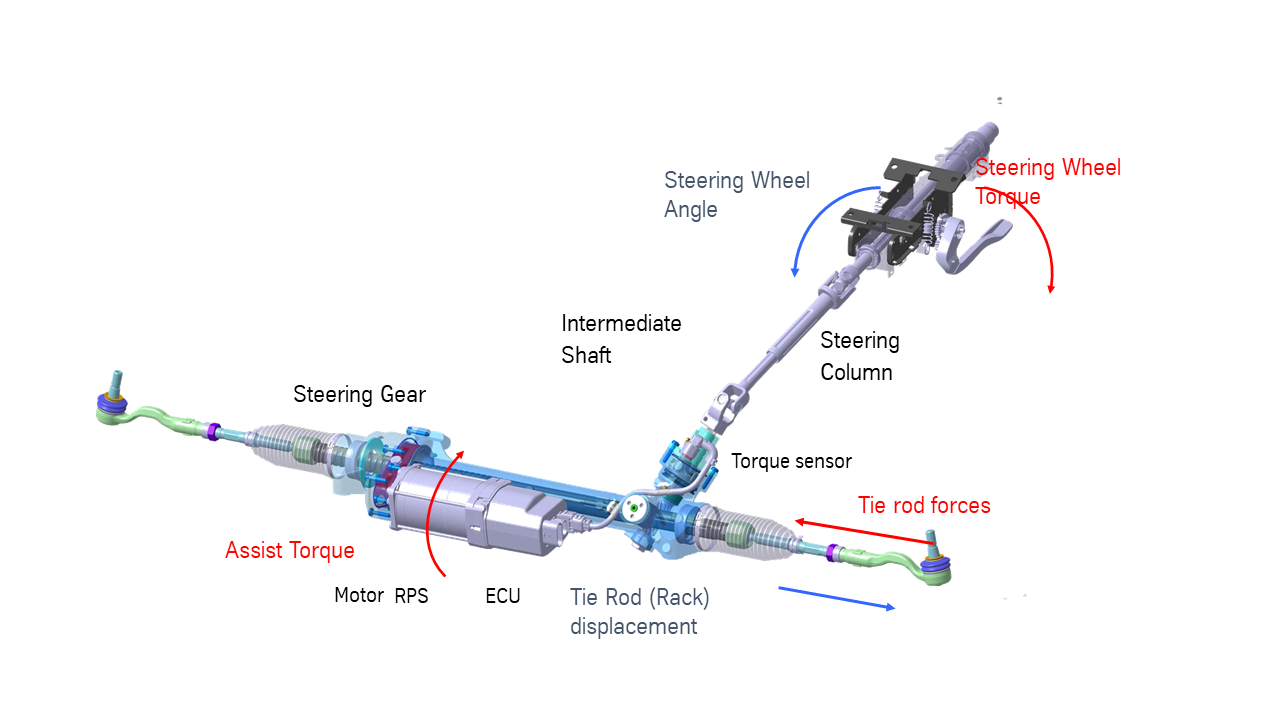
\includegraphics[width=105mm]{figures/parpas_model.png}
		\caption{Model of the parallel-mounted EPAS system~\citep{benyo2013eps}.}
		\label{fig_parpas_model}
	\end{center}
\end{figure}

%~~~~~~~~~~~~~~~~~~~~~~~~~~~~~~~~~~~~~~~~~~~~~~~~~~~~~~~~~~~~~~~~~~~~~~~~~~~~~~~~~
\section{Model reduction}
\label{sec_model_reduction}

In control design, reduced linear models are used to ease the design and simplify complex systems like the steering system of a car.

In order to obtain the simplified linear model with 2 degrees of freedom, the inertia of the wheel, rack, ball screw, tie rods, and motor has to be reduced to the pinion. The related disturbances, frictions, and damping also have to be transferred to the pinion.

The motor inertia is reduced to the pinion as follows:

\begin{align}
	\begin{split}
		J_{red} = J_{motor} 
		\cdot \Bigg( \frac{i_{belt} \cdot i_{screw}}{i_{pinion}} \Bigg)^{2} 
		+ J_{screw} \cdot \Bigg( \frac{i_{screw}}{i_{pinion}} \Bigg)^{2} \\
		+ (m_{rack} + m_{tierods}) \cdot \Bigg( \frac{1}{i_{pinion}} \Bigg)^{2} \\
		+ 2 \cdot J_{wheel} \cdot 
		\Bigg( \frac{1}{i_{frame} \cdot i_{pinion}} \Bigg)^{2}
	\end{split}
\end{align}

The motor damping is reduced to the pinion as follows:

\begin{align}
	b_{red} 
	= b_{motor} \cdot \Bigg(\frac{i_{belt} \cdot i_{screw}}{i_{pinion}}\Bigg)^{2}
	+ b_{screw} \cdot \Bigg(\frac{i_{screw}}{i_{pinion}}\Bigg)^{2} 
	+ b_{rack} \cdot \Bigg(\frac{1}{i_{pinion}}\Bigg)^{2}
\end{align}

The result of this model reduction is the simplified linear model, which is a damped mass-spring system with two degrees of freedom as shown in Figure~\ref{fig_red_lin_model}.

The following symbols are used as notations in the figure: The $J_{up}$ is the reduced inertia of the motor, screw, wheel, rack, and tie rods, and the $J_{red}$ is the inertia of the steering wheel. In between them, there are the steering column inner damping ($b_{sensor}$) and the steering column stiffness ($c_{sensor}$), which primarily consists of the torque sensor (torsion bar) stiffness. The $b_{up}$ viscous coefficient of the steering wheel friction; the $b{red}$ is the reduced damping of the motor, screw, and rack.

The system input is the required motor torque ($T_{motor}$), and the disturbances are the driver torque ($T_{driver}$) and the load ($T_{load}$). The measurements of the system are the outputs. The motor angle speed ($i_{gear} \cdot \omega_{pinion}$), and the steering column torque ($c_{sensor} \cdot \Delta \varphi$).

\begin{figure}[b]
	\begin{center}
		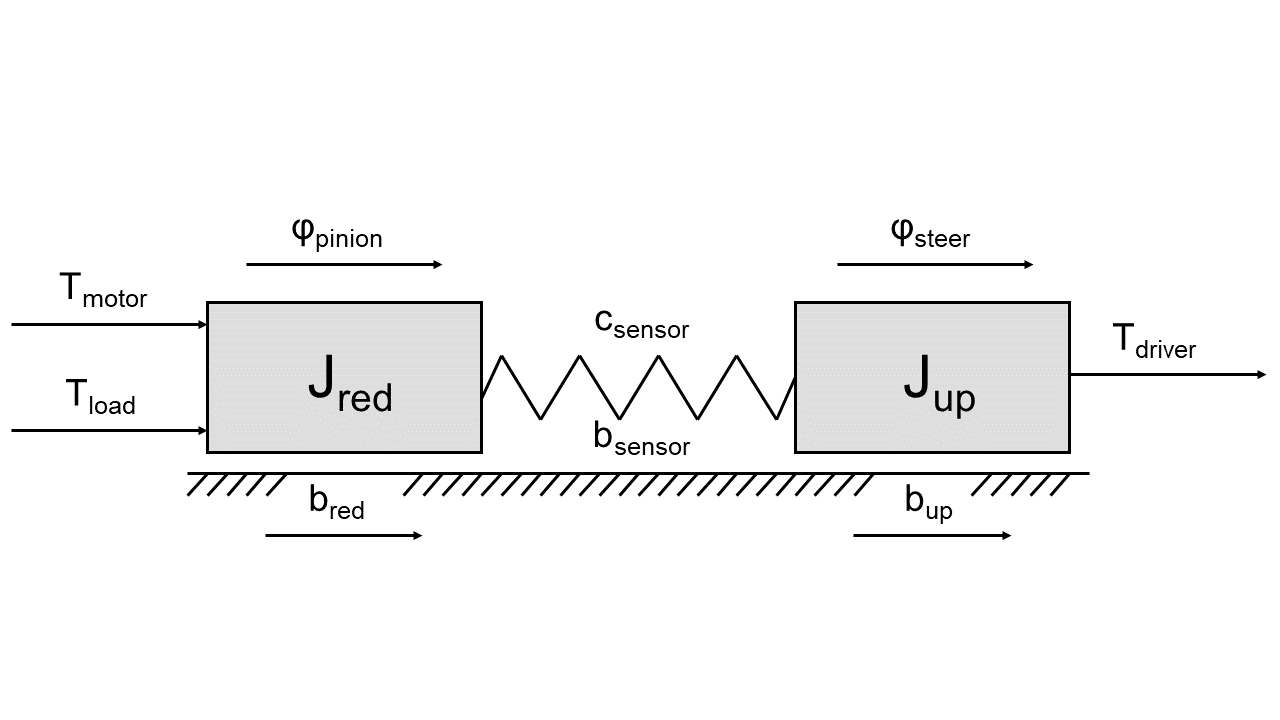
\includegraphics[width=100mm]{figures/red_lin_model.png}
		\caption{Reduced linear model of the EPAS 
		system~\citep{paholics2006epas}.}
		\label{fig_red_lin_model}
	\end{center}
\end{figure}

 %TODO EPAS INTRO

%~~~~~~~~~~~~~~~~~~~~~~~~~~~~~~~~~~~~~~~~~~~~~~~~~~~~~~~~~~~~~~~~~~~~~~~~~~~~~~~~~
\chapter{Affine Lyapunov function candidates for the EPAS LPV model}
% Approx. 5 pages


%----------------------------------------------------------------------------
\chapter{Analysis of the quadratic stability regions of the EPAS LPV model}
% Approx. 5 pages
%----------------------------------------------------------------------------


%----------------------------------------------------------------------------
\chapter{Conclusion}
%----------------------------------------------------------------------------
 %TODO

\listoffigures\addcontentsline{toc}{chapter}{\listfigurename}

\listoftables\addcontentsline{toc}{chapter}{\listtablename}

%~~~~~~~~~~~~~~~~~~~~~~~~~~~~~~~~~~~~~~~~~~~~~~~~~~~~~~~~~~~~~~~~~~~~~~~~~~~~~~~~~~~~~~
\appendix
%~~~~~~~~~~~~~~~~~~~~~~~~~~~~~~~~~~~~~~~~~~~~~~~~~~~~~~~~~~~~~~~~~~~~~~~~~~~~~~~~~~~~~~
\chapter*{\fuggelek}\addcontentsline{toc}{chapter}{\fuggelek}
\setcounter{chapter}{\appendixnumber}
%\setcounter{equation}{0} % a fofejezet-szamlalo az angol ABC 6. betuje (F) lesz
\numberwithin{equation}{section}
\numberwithin{figure}{section}
\numberwithin{lstlisting}{section}
%\numberwithin{tabular}{section}
%~~~~~~~~~~~~~~~~~~~~~~~~~~~~~~~~~~~~~~~~~~~~~~~~~~~~~~~~~~~~~~~~~~~~~~~~~~~~~~~~~~~~~~

\section{Norms on matrices, signals and systems}

In this complementary section, some important notations about matrix, system, and signal norms are given. 
The definition presented hereafter is mainly based on \citep{bronshtein2013handbook} \citep{vizer2015thesis}.

Let us first consider a vector or a signal space denoted by \textit{X}. Then a norm on \textit{X} can be defined as follows:

\definition 
A norm is real valued function $\|\bullet\|$ on X fulfilling the following properties:
%
\begin{subequations}
%
	\begin{align}
		&\text{Positivity} & &\rightarrow & 
		\|x\| &\geq 0 \\
		&\text{Positive Definities} & &\rightarrow &
		\|x\| &\geq 0, \|x\| = 0 \Leftrightarrow x = 0 \\
		&\text{Homogeneity} & &\rightarrow & 
		\|cx\| &= |c| \|x\|, c \in \mathbb{R} \\
		&\text{Triangle Inequality} & &\rightarrow & 
		\|x + y\| &\leq \|x\| + \|y\|
	\end{align}
%	
	\begin{itemize}
		\item[] for any $x,y \in X$.
	\end{itemize}
%
\end{subequations}

See \citep[Chapter~4]{bronshtein2013handbook}, for further information about signals and vector spaces \citep{vizer2015thesis}.

%~~~~~~~~~~~~~~~~~~~~~~~~~~~~~~~~~~~~~~~~~~~~~~~~~~~~~~~~~~~~~~~~~~~~~~~~~~~~~~~~~~~~~~

\subsection{Matrix norms}

Let us consider an $n \times m$ matrix $\mathcal{A} \in \mathbb{R}^{n \times m}$. 
Then the following norms can be defined:
%
\begin{subequations} \label{MatrixNorms}
	\begin{itemize}
%
		\item \textbf{1-norm:}
			\begin{align} 
				\|\mathcal{A}\|_1 &= 
				\underset{\substack{j}}{max} \underset{\substack{i}}{\sum} |a_{ij}|
			\end{align}
%			
		\item \textbf{2-norm:} 
			\begin{align}
				\|\mathcal{A}\|_2 &= \sqrt{\lambda_1 (A^T A)}
			\end{align}
%			
		\item[] where $\lambda_1 (\bullet)$ and $(\bullet)^T$ are the maximal 
		eigenvalue function and the transpose of $\bullet$, respectively;
%		
		\item \textbf{$\infty$-norm:} 
			\begin{align}
				\|\mathcal{A}\|_{\infty} &= 
				\underset{\substack{i}}{max} \underset{\substack{j}}{\sum}|a_{ij}|
			\end{align}
%			
		\item \textbf{Frobenius-norm:}
			\begin{align}
				\|\mathcal{A}\|_F &= 
				\sqrt{\underset{\substack{ij}}{\sum}|a_{ij}|^2} = \sqrt{Tr(A A^H)} 
			\end{align}	
%			
		\item[] where, $Tr(\bullet)$ and $(\bullet)^H$ are the sum of the main 
		diagonal elements of an $n \times n$ matrix and the Hermitian transpose of 
		$\bullet$, respectively \citep{bronshtein2013handbook}.
%
	\end{itemize}
\end{subequations}

%~~~~~~~~~~~~~~~~~~~~~~~~~~~~~~~~~~~~~~~~~~~~~~~~~~~~~~~~~~~~~~~~~~~~~~~~~~~~~~~~~~~~~~

\subsection{Signal norms}

Throughout this work, we consider square-integrable, piece-wise continuous functions such that
%
\begin{align}
	f(x),t \in \mathbb{R} =  
		\begin{cases}
			f(t) \geq 0	& \text{if } t \geq 0 \\
			f(t) = 0 & \text{if } t < 0 \\
			\int_{-\infty}^{\infty}|f(t)|^2dt < \infty &
		\end{cases}
\end{align}

Then the following norms can be defined:
%
\begin{subequations} \label{SignalNorms}
	\begin{itemize}
%	
		\item \textbf{$\mathcal{L}_1$-norm:}
			\begin{align}
				\|f\|_1 &= 
				\int_{-\infty}^{\infty}|f(t)| dt
			\end{align}
%			
		\item \textbf{$\mathcal{L}_2$-norm:}
			\begin{align}
				\|f\|_2 &= 
				\Bigg(\int_{-\infty}^{\infty}f(t)^2 dt\Bigg)^{1/2}
			\end{align}
%			
		\item \textbf{$\mathcal{L}_p$-norm:}
			\begin{align}
				\|f\|_p &= 
				\Bigg(\int_{-\infty}^{\infty}f(t)^p dt\Bigg)^{1/p}
			\end{align}
%			
		\item \textbf{$\mathcal{L}_\infty$-norm:}
			\begin{align}
				\|f\|_{\infty} &= 
				\underset{\substack{t}}{sup}|f(t)|
			\end{align}
%
	\end{itemize}
\end{subequations}

%~~~~~~~~~~~~~~~~~~~~~~~~~~~~~~~~~~~~~~~~~~~~~~~~~~~~~~~~~~~~~~~~~~~~~~~~~~~~~~~~~~~~~~

\subsection{System norms}

During this thesis, system norms are defined for stable, causal, finite-dimensional, time-invariant systems (see \citep{kailath1980linear} for further details). 
A system is a mapping between two signals having the following convolution equation:
%
\begin{subequations}
%
	\begin{align}
		y(t)=g(t) \ast u(t),
	\end{align}
%	
	\begin{itemize}
		\item[] which can be written as
	\end{itemize}
%	
	\begin{align}
		y(t)=\int_{-\infty}^{\infty}g(t - \tau) u(\tau) d\tau.
	\end{align}
%
\end{subequations}

Let us denote $\mathcal{G}(s)$, the Laplace transform of $g(t)$, which is the so-called transfer function. Thus, $\mathcal{G}(s)$ is analytic in the closed right half-complex plane, fulfilling the stability property \citep{kailath1980linear}. By replacing the Laplace variables $s$ with $j\omega$, it can further be concluded that $\mathcal{G}(s)$ is proper if $\mathcal{G}(j\infty)$ is finite, and strictly proper if $\mathcal{G}(j\infty) = 0$. 

Two norms for the transfer function $\mathcal{G}(s)$ can now be defined:
%
\begin{subequations} \label{SystemNorms}
	\begin{itemize}
%	
		\item \textbf{$\mathcal{H}_2$-norm:}
			\begin{align}
				\|\mathcal{G}\|_2 &= 
				\Bigg( \frac{1}{2\pi} \int_{-\infty}^{\infty}
				|\mathcal{G}(j\omega)|^2 dt \Bigg)^{1/2}
			\end{align}
%			
		\item \textbf{$\mathcal{H}_\infty$-norm:}
			\begin{align}
				\|\mathcal{G}\|_\infty &= 
				\underset{\substack{\omega}}{sup}|\mathcal{G}(j\omega)| = 
				\sigma_1(\mathcal{G}(j\omega))
			\end{align}
%			
		\item[] where, $\sigma_1(\mathcal{G}(j\omega))$ denotes the 
		maximal singular value of the transfer function 
		$\mathcal{G}(j\omega)$ \citep{vizer2015thesis}.
%		
	\end{itemize}
\end{subequations}

%~~~~~~~~~~~~~~~~~~~~~~~~~~~~~~~~~~~~~~~~~~~~~~~~~~~~~~~~~~~~~~~~~~~~~~~~~~~~~~~~~~~~~~

%~~~~~~~~~~~~~~~~~~~~~~~~~~~~~~~~~~~~~~~~~~~~~~~~~~~~~~~~~~~~~~~~~~~~~~~~~~~~~~~~~~~~~~

\clearpage \section{A TeXstudio felülete}
\begin{figure}[!ht]
\centering
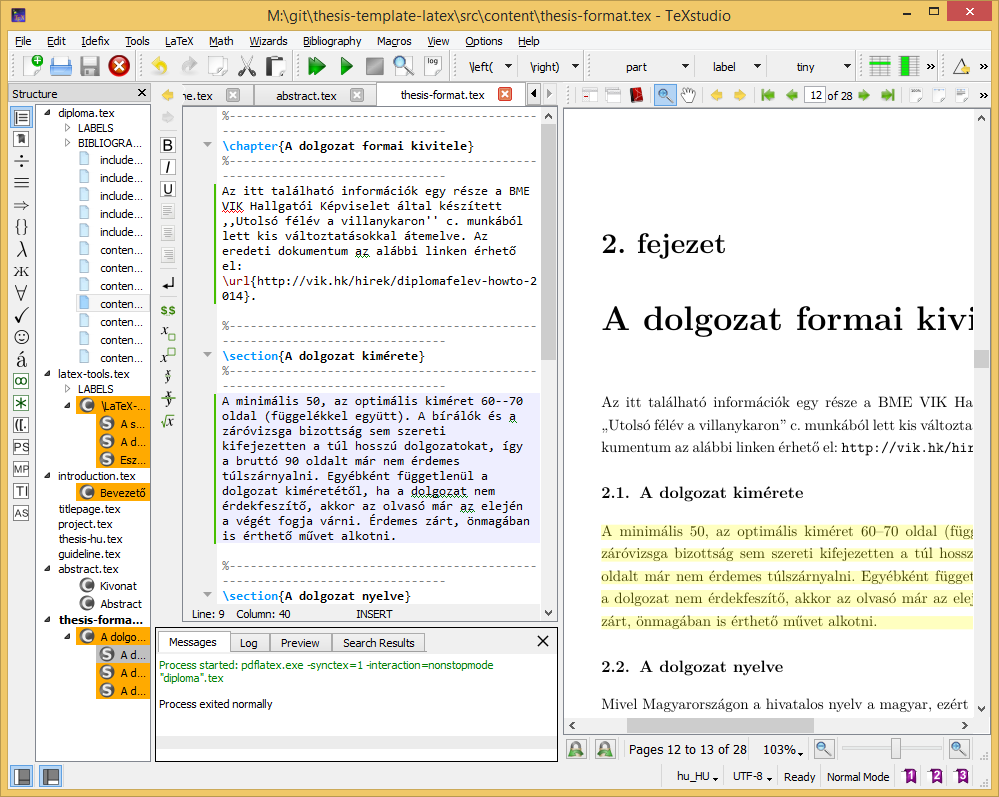
\includegraphics[width=150mm, keepaspectratio]{figures/TeXstudio.png}
\caption{A TeXstudio \LaTeX-szerkesztő.} 
\end{figure}
 %TODO

%Bibliography ~ To solve the bib problem F6 F11 F6 F6, then F7 (view pdf).
\addcontentsline{toc}{chapter}{\bibname}

\bibliography{bib/mybib}

%\label{page:last}
\end{document}